%! app: Regular Languages
%! outcome: Formal definition of automata, Informal definition of automata, Nondeterminism


\begin{comment}

\vfill
Let  $\Sigma = \{a,b\}$. A state diagram for a DFA that recognizes 
$\{w \mid w~\text{has $ab$ as a substring and is of even length} \}$:


\vfill


Suppose $A_1, A_2$ are languages over an alphabet $\Sigma$.
{\bf Claim:} if there is a DFA $M_1$ such that $L(M_1) = A_1$ and 
DFA $M_2$ such that $L(M_2) = A_2$, then there is another DFA, let's call it $M$, such that 
$L(M) = A_1 \cap A_2$.

{\bf Proof idea}:


{\bf Formal construction}: 


\vspace{70pt}

{\bf Application}:  When $A_1 = \{w \mid w~\text{has $ab$ as a substring} \}$ and 
$A_2 = \{ w \mid w~\text{is of even length} \}$.


\newpage

Suppose $A_1, A_2$ are languages over an alphabet $\Sigma$.
{\bf Claim:} if there is a DFA $M_1$ such that $L(M_1) = A_1$ and 
DFA $M_2$ such that $L(M_2) = A_2$, then there is another DFA, let's call it $M$, such that 
$L(M) = A_1 \cup A_2$.  {\it Sipser Theorem 1.25, page 45}

{\bf Proof idea}:


{\bf Formal construction}: 

\vspace{70pt}

{\bf Application}: A state diagram for a DFA that recognizes $\{w \mid w~\text{has $ab$ as a substring or is of even length} \}$:

\vspace{100pt}
\end{comment}

The state diagram of an NFA over $\{a,b\}$ is below.  The formal definition of this NFA is:

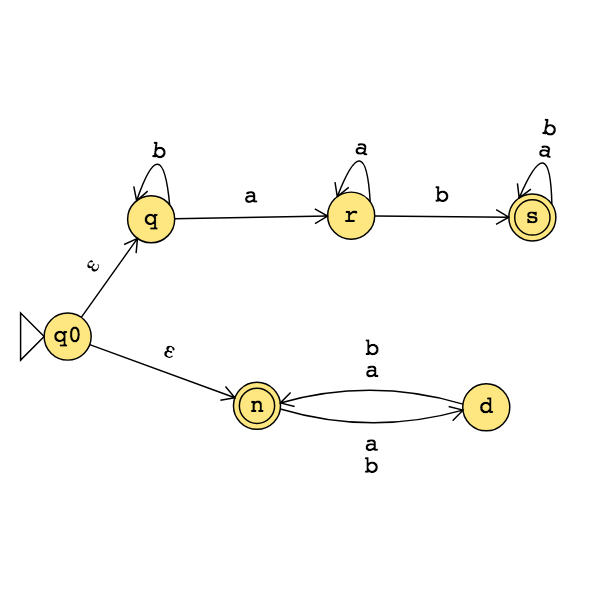
\includegraphics[width=2.5in]{../../resources/machines/Lect5NFA1.png}

The language recognized by this NFA is: 



Suppose $A_1, A_2$ are languages over an alphabet $\Sigma$.
{\bf Claim:} if there is a NFA $N_1$ such that $L(N_1) = A_1$ and 
NFA $N_2$ such that $L(N_2) = A_2$, then there is another NFA, let's call it $N$, such that 
$L(N) = A_1 \cup A_2$.

{\bf Proof idea}: Use nondeterminism to choose which of $N_1$, $N_2$ to run.


{\bf Formal construction}: Let 
$N_1 = (Q_1, \Sigma, \delta_1, q_1, F_1)$ and $N_2 = (Q_2, \Sigma, \delta_2,q_2, F_2)$
and assume $Q_1 \cap Q_2 = \emptyset$ and that $q_0 \notin Q_1 \cup Q_2$.
Construct $N = (Q, \Sigma, \delta, q_0, F_1 \cup F_2)$ where
\begin{itemize}
    \item $Q = $
    \item $\delta: Q \times \Sigma_\varepsilon \to \mathcal{P}(Q)$ is defined by, for $q \in Q$ and $a \in \Sigma_{\varepsilon}$:
        \[
            \phantom{\delta((q,a))=\begin{cases}  \delta_1 ((q,a)) &\qquad\text{if } q\in Q_1 \\ \delta_2 ((q,a)) &\qquad\text{if } q\in Q_2 \\ \{q1,q2\} &\qquad\text{if } q = q_0, a = \varepsilon \\ \emptyset\text{if } q= q_0, a \neq \varepsilon \end{cases}}
        \]
\end{itemize}


\vfill
{\it Proof of correctness would prove that $L(N) = A_1 \cup A_2$ by considering
an arbitrary string accepted by $N$, tracing an accepting computation of $N$ on it, and using 
that trace to prove the string is in at least one of $A_1$, $A_2$; then, taking an arbitrary 
string in $A_1 \cup A_2$ and proving that it is accepted by $N$. Details left for extra practice.}

\newpage
Over the alphabet $\{a,b\}$, the language $L$ described by the regular expression 
$\Sigma^* a \Sigma^* b$

 includes the strings \phantom{space for strings here} and excludes the strings 


The state diagram of a NFA recognizing $L$ is:

\vspace{100pt}

Suppose $A_1, A_2$ are languages over an alphabet $\Sigma$.
{\bf Claim:} if there is a NFA $N_1$ such that $L(N_1) = A_1$ and 
NFA $N_2$ such that $L(N_2) = A_2$, then there is another NFA, let's call it $N$, such that 
$L(N) = A_1 \circ A_2$.

{\bf Proof idea}: Allow computation to move between $N_1$ and $N_2$ ``spontaneously" when reach an accepting state of 
$N_1$, guessing that we've reached the point where the two parts of the string in the set-wise concatenation 
are glued together.


{\bf Formal construction}: Let 
$N_1 = (Q_1, \Sigma, \delta_1, q_1, F_1)$ and $N_2 = (Q_2, \Sigma, \delta_2,q_2, F_2)$
and assume $Q_1 \cap Q_2 = \emptyset$.
Construct $N = (Q, \Sigma, \delta, q_0, F)$ where
\begin{itemize}
    \item $Q = $
    \item $q_0 = $
    \item $F = $
    \item $\delta: Q \times \Sigma_\varepsilon \to \mathcal{P}(Q)$ is defined by, for $q \in Q$ and $a \in \Sigma_{\varepsilon}$:
        \[
            \delta((q,a))=\begin{cases}  
                \delta_1 ((q,a)) &\qquad\text{if } q\in Q_1 \textrm{ and } q \notin F_1\\ 
                \delta_1 ((q,a)) &\qquad\text{if } q\in F_1 \textrm{ and } a \in \Sigma\\ 
                \delta_1 ((q,a)) \cup \{q_2\} &\qquad\text{if } q\in F_1 \textrm{ and } a = \varepsilon\\ 
                \delta_2 ((q,a)) &\qquad\text{if } q\in Q_2
            \end{cases}
        \]
\end{itemize}

\vfill

{\it Proof of correctness would prove that $L(N) = A_1 \circ A_2$ by considering
an arbitrary string accepted by $N$, tracing an accepting computation of $N$ on it, and using 
that trace to prove the string can be written as the result of concatenating two strings, 
the first in $A_1$ and the second in $A_2$; then, taking an arbitrary 
string in $A_1 \circ A_2$ and proving that it is accepted by $N$. Details left for extra practice.}

\newpage

Suppose $A$ is a language over an alphabet $\Sigma$.
{\bf Claim:} if there is a NFA $N$ such that $L(N) = A$, then there is another NFA, let's call it $N'$, such that 
$L(N') = A^*$.

{\bf Proof idea}: Add a fresh start state, which is an accept state. Add spontaneous 
moves from each (old) accept state to the old start state.

{\bf Formal construction}: Let 
$N = (Q, \Sigma, \delta, q_1, F)$ and assume $q_0 \notin Q$.
Construct $N' = (Q', \Sigma, \delta', q_0, F')$ where
\begin{itemize}
    \item $Q' = Q \cup \{q_0\}$
    \item $F' = F \cup \{q_0\}$
    \item $\delta': Q' \times \Sigma_\varepsilon \to \mathcal{P}(Q')$ is defined by, for $q \in Q'$ and $a \in \Sigma_{\varepsilon}$:
        \[
            \delta'((q,a))=\begin{cases}  
                \delta ((q,a)) &\qquad\text{if } q\in Q \textrm{ and } q \notin F\\ 
                \delta ((q,a)) &\qquad\text{if } q\in F \textrm{ and } a \in \Sigma\\ 
                \delta ((q,a)) \cup \{q_1\} &\qquad\text{if } q\in F \textrm{ and } a = \varepsilon\\ 
                \{q_1\} &\qquad\text{if } q = q_0 \textrm{ and } a = \varepsilon \\
                \emptyset &\qquad\text{if } q = q_0 \textrm { and } a \in \Sigma
            \end{cases}
        \]
\end{itemize}


{\it Proof of correctness would prove that $L(N') = A^*$ by considering
an arbitrary string accepted by $N'$, tracing an accepting computation of $N'$ on it, and using 
that trace to prove the string can be written as the result of concatenating some number of strings, 
each of which is in $A$; then, taking an arbitrary 
string in $A^*$ and proving that it is accepted by $N'$. Details left for extra practice.}


{\bf Application}: A state diagram for a NFA over $\Sigma = \{a,b\}$ 
that recognizes $L (( \Sigma^* b)^* )$:

\vspace{200pt}




{\bf True} or {\bf False}: The state diagram of any DFA is also the state diagram of a NFA.

{\bf True} or {\bf False}: The state diagram of any NFA is also the state diagram of a DFA.

{\bf True} or {\bf False}: The formal definition $(Q, \Sigma, \delta, q_0, F)$ of any DFA is also the formal definition of a NFA.

{\bf True} or {\bf False}: The formal definition $(Q, \Sigma, \delta, q_0, F)$  of any NFA is also the formal definition of a DFA.

